\chapter{Spazi metrici}
\section{Insiemi e distanze}
Uno spazio metrico è un insieme generico in cui è definito il concetto di distanza, che è una funzione che rispetta delle proprietà ben definite e ad ogni coppia di numeri associa un numero (reale) che è sempre positivo o nullo, in modo simmetrico.
\begin{definizione}
Sia $X$ un insieme qualunque e $d$ una funzione, detta distanza, del tipo
\[
d\colon X\times X\to\R,
\]
che soddisfa le seguenti proprietà $\forall x,y,z\in X$:
\begin{enumerate}
\item $d(x,y)\geq 0$, e in particolare $d(x,y)=0\iff x=y$;
\item $d(x,y)=d(y,x)$, cioè è simmetrica;
\item $d(x,y)\leq d(x,z)+d(z,y)$ (disuguaglianza triangolare).
\end{enumerate}
L'insieme $X$ associato alla distanza $d$ è detto \emph{spazio metrico} e si indica con $(X,d)$.
\end{definizione}
In generale, per ogni spazio metrico si può definire più di un tipo di distanza.
\begin{esempio} \label{es:distanze}
	Ecco alcuni esempi di distanze, alcune delle quali ritroveremo più avanti.
	\begin{enumerate}
		\item La distanza euclidea è definita dalla norma, come nella definizione \ref{d:norma}, che per $\R$ (o anche $\Q$), essendo in un'unica dimensione, si riduce a $\norm{\vec x-\vec y}=\abs{x-y}$.
		\item La distanza $d_\infty$ in $\R^2$ è definita come il massimo delle distanze delle coordinate omologhe: $d_\infty(\vec x,\vec y)=\max\{\abs{x_1-y_1},\abs{x_2-y_2}\}$.
		\item La distanza $d_1(\vec x,\vec y)=\abs{x_1-y_1}+\abs{x_2-y_2}$ in $\R^2$ è la somma delle distanze tra le componenti omologhe.
		\item Nello spazio $X=\{\phi\colon[a,b]\to\R\colon\phi\text{ è limitata}\}$ la distanza tra due funzioni $f$ e $g$ definite in un intervallo $[a,b]$ e in cui sono limitate, cioè se $f\big([a,b]\big)$ e $g\big([a,b]\big)$ sono insiemi limitati, è definita come $d_*(f,g)=\sup_{x\in[a,b]}\abs{f(x)-g(x)}$.
		\item La metrica \emph{discreta}, in un insieme qualsiasi, è definita dalla distanza
			\[
				d_D(x,y)=
				\begin{cases*}
					0 &se $x=y$,\\
					1 &se $x\neq y$.
				\end{cases*}
			\]
	\end{enumerate}
\end{esempio}
\begin{definizione}
Sia $(X,d)$ uno spazio metrico. Dati un punto $p\in X$ e $r>0$, si chiama \emph{intorno circolare} (o \emph{bolla}) di centro $p$ e raggio $r$ l'insieme
\[
B(p,r)=\{x\in X\colon d(x,p)<r\}.
\]
\end{definizione}
\begin{esempio} \label{es:intorni}
	Ecco alcuni intorni dati dalle distanze che abbiamo definito nell'esempio \ref{es:distanze}.
	\begin{enumerate}
		\item In $(\R,\abs{\cdot})$, gli intorni sono della forma $B=\{x\in\R\colon\abs{x-p}<r\}$, che è l'intervallo aperto $(p-r,p+r)$ (figura \ref{fig:intorno-circolare-r1}).
			\begin{figure}
	\tikzsetnextfilename{intorno-circolare-r1}
	\centering
	\begin{tikzpicture}
		\draw[-|] (-5,0) -- (-2,0) node[above]{$p-r$};
		\draw[-|] (-2,0) -- (0,0) node[above]{$p$};
		\draw[-|] (0,0) -- (2,0) node[above]{$p+r$};
		\draw[->] (0,0) -- (5,0) node[above]{};
		\draw[dashed,|-|] (-2,-.1) -- (2,-.1);
		\draw[fill=black] (0,-.1) circle (.05);
	\end{tikzpicture}
	\caption{Intorno circolare in $\R$ con la distanza data dal valore assoluto.}
	\label{fig:intorno-circolare-r1}
\end{figure}

		\item In $(\R^2,\norm{\cdot})$, gli intorni sono della forma $B=\{\vec x\in\R^2\colon\norm{\vec x-\vec p}<r\}$, che rappresenta un cerchio, privato della circonferenza, di centro $p$ e raggio $r$ (figura \ref{fig:B-circ}).
			\begin{figure}
	\tikzsetnextfilename{intorno-circolare-r2}
	\centering
	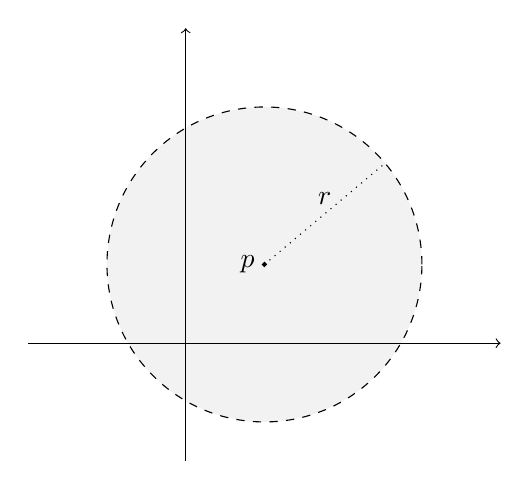
\begin{tikzpicture}
		\draw[dashed,fill=gray!10] (0,0) circle (2);
		\draw[->] (-3,-1) -- (3,-1);
		\draw[->] (-1,-2.5) -- (-1,3);
		\draw (0,0) node[left]{$p$};
		\draw[fill=black] (0,0) circle (.025);
		\draw[dotted] (0,0) to node[anchor=south]{$r$} (40:2);
	\end{tikzpicture}
	\caption{Un intorno $B(\vec p,r)\subset(\R^2,\norm{\cdot})$.}
	\label{fig:B-circ}
\end{figure}

		\item In $(\R^3,\norm{\cdot})$, analogamente al punto precedente, gli intorni sono delle sfere di centro $p$ e raggio $r$, private della superficie sferica.
		\item Con la distanza $d_\infty$, l'intorno $B(\vec 0,r)=\{\vec x\in\R^2\colon\max\{\abs{x_1},\abs{x_2}\}<r\}$ ha la forma di un quadrato di lato $2r$ centrato nell'origine (figura \ref{fig:B-dinfty}).
		\begin{figure}
	\tikzsetnextfilename{intorno-dinfty-r2}
	\centering
	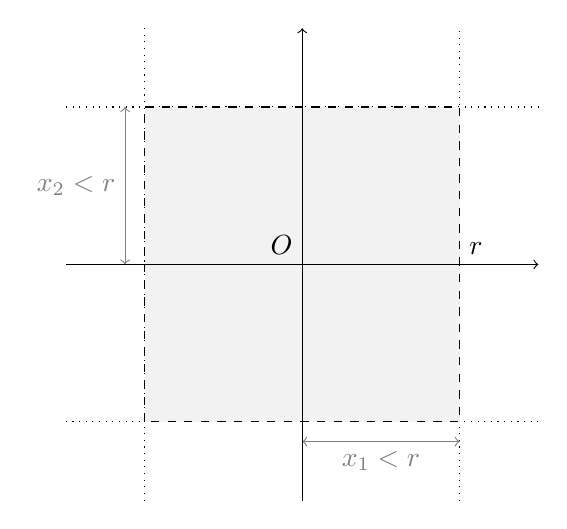
\begin{tikzpicture}
		\draw[dotted] (-3,2) -- (3,2);
		\draw[dotted] (3,-2) -- (-3,-2);
		\draw[dotted] (2,-3) -- (2,0) node[above right]{$r$};
		\draw[dotted] (2,0) -- (2,3);
		\draw[dotted] (-2,-3) -- (-2,3);
		\draw[gray,<->] (-2.25,0) to node[gray,anchor=east]{$\abs{x_2}<r$} (-2.25,2);
		\draw[gray,<->] (0,-2.25) to node[gray,anchor=north]{$\abs{x_1}<r$} (2,-2.25);
		\draw[dashed,fill=gray!10] (-2,-2) rectangle (2,2);
		\draw[->] (-3,0) -- (3,0);
		\draw[->] (0,-3) -- (0,3);
		\draw (0,0) node[anchor=south east]{$O$};
	\end{tikzpicture}
	\caption{Un intorno $B(\vec 0,r)\subset(\R^2,d_\infty)$.}
	\label{fig:B-dinfty}
\end{figure}

		\item Con la distanza $d_1$, l'intorno $B(\vec 0,r)=\{\vec x\in\R^2\colon\abs{x_1}+\abs{x_2}<r\}$ ha la forma di un quadrato ruotato di $\pi/4$, di diagonale $2r$ e centrato nell'origine (figura \ref{fig:B-d1}).
		\begin{figure}
	\tikzsetnextfilename{intorno-d1-r2}
	\centering
	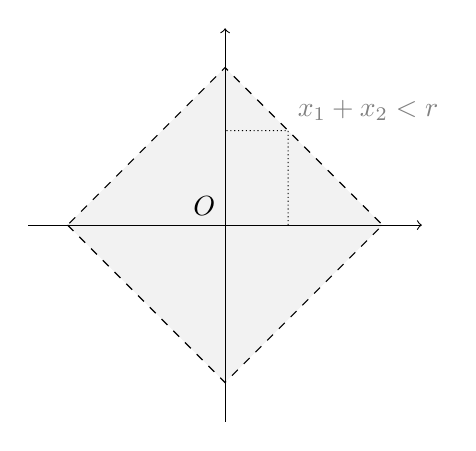
\begin{tikzpicture}
		\filldraw[dashed,fill=gray!10] (-2,0) -- (0,-2) -- (2,0) -- (0,2) -- (-2,0);
		\draw[->] (-2.5,0) -- (2.5,0);
		\draw[->] (0,-2.5) -- (0,2.5);
		\draw[densely dotted] (.8,0) -- (intersection of .8,0--.8,1 and 2,0--0,2) node[gray,anchor=south west]{$\abs{x_1}+\abs{x_2}<r$} -- +(-.8,0);
		\draw (0,0) node[anchor=south east]{$O$};
	\end{tikzpicture}
	\caption{Un intorno $B(\vec 0,r)\subset(\R^2,d_1)$.}
	\label{fig:B-d1}
\end{figure}

		\item Nello spazio $X=\{\phi\colon[a,b]\to\R\colon\phi\text{ è limitata}\}$, con la distanza $d_*$, un intorno di una funzione $f$ è lo spazio limitato dalle funzioni $f-r$ e $f+r$, escluse: $B(f,r)=\{g\in X\colon\sup_{x\in[a,b]}\abs{g(x)-f(x)}<r\}$ (figura \ref{fig:B-d*}).
		\begin{figure}
	\tikzsetnextfilename{intorno-funzione}
	\centering
	\begin{tikzpicture}
		\begin{axis}[standard,xmin=-1,ymin=-1,xmax=7.5,ymax=8,ytick=\empty,xtick={1,6},xticklabels={$a$,$b$},stack plots=y]
			\draw[dotted] (axis cs:1,0) -- (axis cs:1,4.6829);
			\draw[dotted] (axis cs:6,0) -- (axis cs:6,7.4411);
			\draw[gray,<->] (axis cs:3.14,3.14) to node[right]{$r$} (axis cs:3.14,5.14);
			\addplot[draw=none,domain=1:6,samples=200] {-2+x+2*sin(deg(x))};
			\addplot[dashed,domain=1:6,samples=200] {4};
			\addplot[domain=1:6,samples=200] {-2};
			\addplot[dashed,domain=1:6,samples=200] {-2} node[right]{$f-r$};
			\addplot[fill=gray!10,draw=none,domain=1:6,samples=200] {2} node[right]{$f$} \closedcycle;
			\addplot[fill=gray!10,draw=none,dashed,domain=1:6,samples=200] {2} node[right]{$f+r$} \closedcycle;
		\end{axis}
	\end{tikzpicture}
	\caption{Un intorno $B(f,r)\subset(X,d_*)$ della funzione $f=x+2\sin x$.}
	\label{fig:B-d*}
\end{figure}

	\end{enumerate}
\end{esempio}

\begin{teorema}
\label{t:hausdorff}
Siano $p$ e $q$ due punti distinti appartenenti ad uno spazio metrico $(X,d)$. Esiste almeno una coppia di raggi $r_1$ e $r_2$ tali che
\[
B(p,r_1)\cap B(q,r_2)=\emptyset.
\]
\end{teorema}
\begin{proof}
	Sia $d$ la distanza tra i due punti $p,q$. Definito $r_1=r_2=\frac{d}3$ le due bolle hanno intersezione vuota. In generale, qualunque coppia di raggi la cui somma sia minore della distanza dei due punti è adatta a dimostrare il teorema.
\end{proof}
La proprietà per cui $\forall x,y\in X$ esistono degl intorni aperti $U$ di $x$ e $V$ di $y$ tali che $U\cap V=\emptyset$ è detta \emph{proprietà di Hausdorff}: per questo teorema ogni spazio metrico la soddisfa.

\section{Classificazione dei punti}
\begin{definizione}
Siano $(X,d)$ uno spazio metrico e $A\subseteq X$ un suo sottoinsieme. Il punto $p\in X$ si dice
\begin{enumerate}
\item \emph{interno} ad $A$ se esiste una bolla, centrata in $p$, tutta contenuta in tale insieme:
\[
	\exists r>0\colon B(p,r)\subset A;
\]
\item \emph{esterno} ad $A$ se esiste una bolla, centrata in $p$, tutta contenuta nel complementare di tale insieme:
\[
	\exists r>0\colon B(p,r)\subset\compl{A};
\]
\item \emph{di frontiera} se non è interno né esterno, ossia se ogni bolla centrata in $p$ contiene sia punti di $A$ sia del suo complementare:
\[
	\forall r>0,\ B(p,r)\cap A\neq\emptyset\qtext{e}B(p,r)\cap\compl{A}\neq\emptyset.
\]
\end{enumerate}
\end{definizione}
Questa definizione è disgiuntiva ed esaustiva, perché ogni punto rientra sempre in una soltanto delle tre categorie.
L'insieme dei punti interni di $A$ si chiama \emph{interno} e si indica con $\interior{A}$, che non coincide necessariamente con l'insieme stesso. L'insieme dei punti di frontiera, che possono o meno appartenere all'insieme (non si può stabilire a priori) si chiama \emph{frontiera} e si indica con $\boundary A$.
\begin{esempio} \label{es:punti-interni-esterni}
	Applichiamo le definizioni appena date a degli esempi importanti.
	\begin{enumerate}
		\item In ogni spazio metrico $(X,d)$, l'insieme $X$ ha solo punti interni.
		\item Ogni punto è esterno ad un insieme vuoto.
		\item L'interno di un intorno coincide \emph{sempre} con l'intorno stesso.
		\item La frontiera di un intorno $B(\vec p,r)\subset\R^2$ è la circonferenza di raggio $r$, centrata in $\vec p$, cioè $\boundary B=\{\vec x\in\R^2\colon\norm{\vec x-\vec p}=r\}$.
		\item La frontiera dello stesso insieme del punto precedente, ma in $\R^3$, quindi il cerchio $\{\vec x\in\R^3\colon(x_1-p_1)^2+(x_2-p_2)^2<r^2,\ x_3=p_3\}\subset\R^3$ è \emph{l'insieme stesso}, e non più la sua circonferenza.
		\item La frontiera di $\Q\subset\R$ è proprio $\R$, perché ogni intorno di un punto razionale contiene infiniti altri punti razionali e irrazionali (gli irrazionali formano il complementare di $\Q$ rispetto ad $\R$). Analogamente, $\R$ è anche la frontiera di $\R\setminus\Q$.
		\item Con la metrica discreta, se $x\in A$, allora $B(x,1)=\{x\}\subseteq A$, mentre se $y\in\compl{A}$ allora $B(y,1)=\{y\}\subseteq\compl{A}$, quindi ogni punto di un insieme è ad esso interno, mentre ogni punto del complementare è esterno. Quindi la frontiera di un insieme è sempre vuota, anche perché qualsiasi intorno di raggio $r\leq 1$ contiene soltanto il punto, che è il centro della bolla, quindi nessun altro punto del'insieme o del complementare.
	\end{enumerate}
\end{esempio}
\begin{osservazione}
Fissati uno spazio metrico $(X,d)$ e un suo sottoinsieme $A$, se un punto $p\in X$ non è esterno a tale insieme, allora ogni bolla centrata in $p$ di qualsiasi raggio non è un sottoinsieme del complementare di $A$, cioè la sua intersezione con $A$ non è mai vuota:
\[
	\forall r>0,\ B(p,r)\not\subset\compl{A},\text{ vale a dire }B(p,r)\cap A\neq\emptyset.
\]
\end{osservazione}
\begin{definizione}
Siano $(X,d)$ uno spazio metrico e $A\subseteq X$ un suo sottoinsieme. Il punto $p\in X$ non esterno ad $A$ si dice
\begin{itemize}
\item \emph{di accumulazione} per $A$, se ogni bolla centrata in $p$ contiene punti di $A$, oltre al centro stesso della bolla:
\[
\forall r>0,\ B(p,r)\cap A\setminus\{p\}\neq\emptyset;
\]
\item \emph{isolato}, se esiste almeno una bolla centrata nel punto che non contiene altri punti dell'insieme, oltre a $p$ stesso:
\[
\exists r>0\colon B(p,r)\cap A=\{p\}.% uguale a {p} o al vuoto?
\]
\end{itemize}
\end{definizione}
L'insieme dei punti di accumulazione di $A$ si chiama \emph{derivato} e si indica con $A'$. Si dimostra inoltre che se l'intorno di un punto di accumulazione contiene almeno un altro punto dell'insieme, ne contiene infiniti.
\begin{teorema}
Siano $(X,d)$ uno spazio metrico e $A\subseteq X$ un suo sottoinsieme. Se $p\in A'$, l'intersezione tra una bolla di qualsiasi raggio e l'insieme $A$ ha cardinalità infinita.
\[
	\forall r>0,\ \card{B(p,r)\cap A}=\infty.
\]
\end{teorema}
\begin{proof}
Si supponga per assurdo che esista un raggio $\tilde{r}$ tale che la bolla centrata in $p$ abbia cardinalità finita, quindi che $\exists\tilde{r}>0\colon B(p,\tilde{r})\cap A=\{x_1,x_2,\dots,x_n\}$. Per ogni punto $x_i$ di questa bolla possiamo individuare la distanza $r_i=d(p,x_i)$ dal centro, per ogni $i=1,2,\dots,n$. Poiché l'insieme di questi raggi $r_i$ è finito (ha precisamente $n$ elementi), l'esistenza del suo minimo è certa. Allora preso un nuovo raggio $r'$ qualunque tale che $r'<\min_{1\leq i\leq n}\{r_i\}$, una nuova bolla centrata in $p$ non conterrà più alcun elemento di $A$, infatti si ha che
\[
B(p,r')\cap A=\{p\},
\]
cioè $p$ è un punto isolato, che è la negazione della tesi. Quindi il teorema è dimostrato.
\end{proof}
\begin{corollario}
In ogni spazio metrico, il derivato di qualsiasi insieme di cardinalità finita è vuoto.
\[
\forall (X,d),\, A\subseteq X,\text{ se $A$ è finito}\then A'=\emptyset.
\]
\end{corollario}
\section{Insiemi aperti, chiusi e limitati}
\begin{definizione}
\label{d:chiuso-se-c-aperto}
Siano $(X,d)$ uno spazio metrico e $A\subseteq X$ un suo sottoinsieme. $A$ si dice
\begin{itemize}
\item \emph{aperto}, se tutti i suoi punti sono interni, quindi $\interior{A}=A$;
\item \emph{chiuso}, se il suo complementare $\compl{A}$ è aperto.
\end{itemize}
\end{definizione}
Questa non è una definizione esaustiva, infatti esistono insiemi che non sono aperti né chiusi. Si dà anche la seguente caratterizzazione, cioè una condizione necessaria e sufficiente.
\begin{teorema}
Siano $(X,d)$ uno spazio metrico e $A\subseteq X$ un suo sottoinsieme. L'insieme $A$ è chiuso se e solo se contiene i suoi punti di accumulazione.
\[
A\text{ è chiuso}\iff A'\subseteq A.
\]
\end{teorema}
\begin{proof}
(i) Se $A$ è chiuso, contiene i suoi punti di accumulazione.
Sia $p\in \compl{A}$, che quindi per ipotesi, dato che $A$ è chiuso, è aperto. Allora esiste una bolla centrata in $p$ tutta contenuta in $\compl{A}$: quindi l'intersezione di tale bolla con l'insieme $A$ deve essere vuota, e $p$ non può essere un punto di accumulazione di $A$.
\[
\exists r>0\colon B(p,r)\subset \compl{A}\qqq B(p,r)\cap A=\emptyset\qqq p\notin A'.
\]
Necessariamente allora i punti di accumulazione devono trovarsi in $A$.

(ii) Se $A$ contiene i suoi punti di accumulazione, è chiuso.
Sia $A'\subseteq A$ e $p$ un qualsiasi punto del complementare. Per ipotesi $p$ non è di accumulazione per $A$, quindi esiste una bolla $B(p,r)$ che non contiene altri punti di $A$ oltre a $p$ stesso. Poiché $p\in \compl{A}$, tale bolla non contiene alcun punto di $A$: allora $B(p,r)\subseteq \compl{A}$, vale a dire $p$ è interno ad $\compl{A}$. Quindi $\compl{A}$ è aperto, a cui segue che $A$ è chiuso.
\end{proof}
\begin{esempio} \label{es:aperti-chiusi}
	Seguono alcuni semplici e comuni esempi per quanto abbiamo appena visto.
	\begin{enumerate}
		\item Ogni intervallo $(a,b)\subset\R$ è aperto, così come $(a,+\infty)$ e $(-\infty,b)$. Analogamente, $[a,b]$, $[a,+\infty)$ e $(-\infty,b]$ sono chiusi. Intervalli del tipo $[a,b)$ non sono aperti né chiusi.
		\item In ogni spazio metrico $(X,d)$, l'insieme $X$ è aperto perché tutti i suoi punti sono interni. Però $X$ è allo stesso tempo anche chiuso, perché contenendo tutti i punti non può che contenere anche quelli di accumulazione di $X'$. Allora $X$ è sia aperto che chiuso, e quindi anche un insieme vuoto è sia aperto che chiuso. 
		\item Ogni intorno è aperto, per definizione, perché tutti i suoi punti sono interni.
		\item In uno spazio metrico discreto, ogni insieme $A\subseteq X$ è aperto, perché ogni suo punto è interno, ma allo stesso tempo tutti i punti sono isolati, quindi $A'=\emptyset$, quindi $A$ (che ovviamente contiene l'insieme vuoto) è anche chiuso.
	\end{enumerate}
\end{esempio}
\begin{teorema} \label{t:unione-intersezione-aperti}
Siano $(X,d)$ uno spazio metrico e $\{A_i\}_{i\in I}$ una famiglia qualunque di sottoinsiemi aperti di tale spazio metrico. Allora
\begin{enumerate}
\item\[
A=\bigcup_{i\in I} A_i\text{ è aperto};
\]
\item se la famiglia è finita, cioè sia $\{A_1,A_2,\dots,A_n\}$, allora
\[
A=\bigcap_{i=1}^n A_i\text{ è aperto}.
\]
\end{enumerate}
\end{teorema}
\begin{proof}
\begin{enumerate}
\item Sia $p$ appartenente ad $A$, l'insieme unione di tutti gli insiemi della famiglia: questo punto deve allora appartenere ad almeno uno degli insiemi della famiglia, cioè $\exists k\colon p\in A_k$. Poiché tutti questi insiemi sono aperti, $p$ è interno a questo insieme $A_k$, quindi esiste una bolla contenuta tutta in questo insieme, la quale allora è anche contenuta nell'insieme unione: $B(p,r)\subset A_k\subset A$.
\item Sia $p$ un punto appartenente ad $A$, l'insieme intersezione degli insiemi appartenenti alla famiglia finita: questo punto deve allora appartenere a ciascuno degli insiemi della famiglia $A_i,\,\forall i$. Ognuno di questi insiemi è aperto, quindi esiste un raggio tale che la bolla centrata in $p$ sia contenuta in ogni insieme, $\exists r_i\colon \forall i\;B(p,r_i)\subset A_i$. Preso $r'=\min\{r_i\}$, la cui esistenza è garantita dal fatto che la famiglia di insiemi è finita, allora la bolla di raggio $r'$ è contenuta in tutti gli insiemi, quindi anche nell'insieme intersezione: $B(p,r')\subset A$.
\end{enumerate}
\end{proof}
In generale, l'intersezione infinita di aperti non è aperta: ad esempio, sia $A_i=(0,1+\frac1{k})$, per $i\in\N$, l'intersezione dà come risultato $\bigcap_{i=1}^{+\infty}A_i=(0,1]$, che non è aperto né chiuso.
Vale anche il seguente teorema, la cui dimostrazione si ricava dal precedente.
\begin{teorema} \label{t:unione-intersezione-chiusi}
Siano $(X,d)$ uno spazio metrico e $\{C_j\}_{j\in J}$ un una famiglia qualunque di sottoinsiemi chiusi di tale spazio metrico. Allora
\begin{enumerate}
\item\[
C=\bigcap_{j\in J} C_j\text{ è chiuso};
\]
\item se la famiglia è finita, cioè sia $\{C_1,C_2,\dots,C_n\}$, allora
\[
C=\bigcup_{j=1}^n C_j\text{ è chiuso}.
\]
\end{enumerate}
\end{teorema}
\begin{proof}
\begin{enumerate}
\item Passando ai complementari dei risultati del teorema precedente, per le formule di De Morgan si ha
\[
	\compl{C}=\compl{\bigg(\bigcap_{j\in J} C_j\bigg)}=\bigcup_{j\in J}\compl{C_j},
\]
che è l'unione di infiniti insiemi aperti, che per il teorema precedente è aperta. Allora $C$ è chiuso, per la definizione \ref{d:chiuso-se-c-aperto}.
\item Analogamente, si ha
\[
	\compl{C}=\compl{\bigg(\bigcup_{j=1}^n C_j\bigg)}=\bigcap_{j=1}^n\compl{C_j},
\]
che è l'intersezione di un numero finito di insiemi aperti, che quindi per il teorema precedente è aperto. Allora $C$ è chiuso, sempre per la \ref{d:chiuso-se-c-aperto}.\qedhere
\end{enumerate}
\end{proof}
Analogamente al controesempio precedente, l'unione di infiniti chiusi non è sempre chiusa: se $C_j=[0,1-\frac1{k}]$ con $j\in\N$, si ha che $\bigcup_{j=1}^{+\infty}C_j=[0,1)$ che non è chiuso, e nemmeno aperto.
\begin{definizione}
Siano $(X,d)$ uno spazio metrico e $A\subseteq X$ un suo sottoinsieme. Si chiama \emph{chiusura} di $A$, e si indica con $\clos{A}$, il più piccolo insieme chiuso che lo contiene. Questo insieme coincide con l'unione dell'insieme stesso con il suo derivato.
\[
\clos{A}=A\cup A'.
\]
\end{definizione}
Si dimostrano che:
\begin{teorema}
Siano $(X,d)$ uno spazio metrico e $A\subseteq X$ un suo sottoinsieme. 
\begin{enumerate}
\item $\clos{A}$ è sempre chiuso;
\item se $F$ è chiuso e $A\subseteq F$, allora $\clos{A}\subseteq F$;
\item se $A$ è chiuso, $\clos{A}=A$ (perché, semplicemente, $A'=A$).
\end{enumerate}
\end{teorema}
\begin{definizione}
Un insieme è \emph{limitato} se esiste, finito, l'estremo superiore delle distanze reciproche tra tutti i suoi elementi.
\[
\sup_{x,y\in A} d(x,y)<+\infty.
\]
Tale estremo superiore è detto \emph{diametro} dell'insieme.
\end{definizione}
Se $A\subseteq (X,d)$ è un insieme limitato, allora il suo diametro coincide con quello della sua chiusura: $\diam A=\diam\clos{A}$; inoltre $\exists p\in X$ e $r>0$ tali per cui $A\subset B(p,r)$, ossia un insieme limitato può essere sempre contenuto in una bolla di opportuno raggio.
\begin{esempio} \label{es:insiemi-limitati}
	Alcuni insiemi limitati e i loro diametri:
	\begin{enumerate}
		\item se $A\subset\R$ un insieme limitato, non vuoto, il suo diametro è dato da $\sup A-\inf A$;
		\item con la metrica discreta il diametro di qualsiasi insieme di almeno due punti è sempre 1, quindi ogni insieme è limitato.
	\end{enumerate}
\end{esempio}
